%%%%%%%%%%%%%%%%%%%%%%%%%%%%%%%%%%%%
% Lesson Plan (50 minutes)
%%%%%%%%%%%%%%%%%%%%%%%%%%%%%%%%%%%%
\begin{frame}
    \frametitle{Lesson Plan}
    \begin{itemize}
        \item xx min Lecture: recap linear regression so far (concepts)
        \item xx min R Demonstration: recap linear regression so far (computation/modeling)
        \item xx min Lecture: recap (briefly) our strategies for inference so far (tests, CI, p-values, etc)
        \item xx min Lecture: putting it all together: motivate inference for linear regression, with an example to return to throughout the week
        \item xx min Edfinity quiz: testing for the slope: what should the hypotheses be?
        \item xx min Lecture: review quiz answers, note t-test inference for regression - idea is to make this now a familiar concept
        \item xx min Edfinity quiz: perform a t-test for the slope parameter, step-by-step
        \item xx min R Demonstration: review quiz answers, interpret the test results together
    \end{itemize}
\end{frame}

%%%%%%%%%%%%%%%%%%%%%%%%%%%%%%%%%%%%
% Learning objectives:
%%%%%%%%%%%%%%%%%%%%%%%%%%%%%%%%%%%%
\begin{frame}
    \frametitle{Learning Objectives}
    \begin{itemize}
        \item \textbf{M1, LO1: Classify and Analyze Variables:} Categorize variables based on their types (e.g., numerical/categorical, continuous/discrete, ordinal), assess their association (positive, negative, or independent), and determine which make sense as explanatory vs. response variables.
        \item \textbf{M1, LO3: Use R for Data Management and Exploration:} Utilize R to load, pre-process, and explore data through visualization and summarization techniques.
        \item \textbf{M1, LO4: Visualize and Describe Data Distributions:} Select appropriate visualizations (scatterplots, histograms, box plots, bar plots) to depict data, and describe distributions qualitatively (shape, center, spread, outliers) and quantitatively (mean, median, mode, range, IQR, standard deviation).
        \item \textbf{M5, LO1: Describe and Assess Relationships Between Two Variables:} Describe the association between two numerical variables in a scatter plot in terms of direction, shape (linear or nonlinear), and strength, and assess whether linear regression is an appropriate model.    
        \item \textbf{M5, LO2: Compute and Interpret Correlation and R²:} Compute and interpret correlation coefficients and R² values, while recognizing that correlation does not imply causation. 
        \item \textbf{M5, LO3: Fit and Interpret Linear Models Using Least Squares:} Fit the intercept and slope of a linear model to data using the least squares method, interpret the fitted values, and use the model to predict responses to new inputs.
        \item \textbf{M5, LO4: Explain and Assess Model Fit:} Explain the least squares fitting procedure, assess whether the fit is unduly influenced by any particular points, and distinguish between interpolation and extrapolation in predictions.
        \item \textbf{M5, LO5: Perform Inference for Regression Coefficients:} Use fit summary and parameter estimates (e.g., ˆβ1 and ˆσ2) to perform hypothesis tests or construct confidence intervals for the slope, and interpret the results.
    \end{itemize}
\end{frame}
    
%%%%%%%%%%%%%%%%%%%%%%%%%%%%%%%%%%%%
% TODO: Copy and adapt these slides base on the lesson plan
%%%%%%%%%%%%%%%%%%%%%%%%%%%%%%%%%%%%

\section{Inference for linear regression}

%%%%%%%%%%%%%%%%%%%%%%%%%%%%%%%%%%%%

\subsection{Understanding regression output from software}

%%%%%%%%%%%%%%%%%%%%%%%%%%%%%%%%%%%

\begin{frame}
\frametitle{Nature or nurture?}

{\small In 1966 Cyril Burt published a paper called ``The genetic determination of differences in intelligence: A study of monozygotic twins reared apart?" The data consist of IQ scores for [an assumed random sample of] 27 identical twins, one raised by foster parents, the other by the biological parents.}

\begin{center}
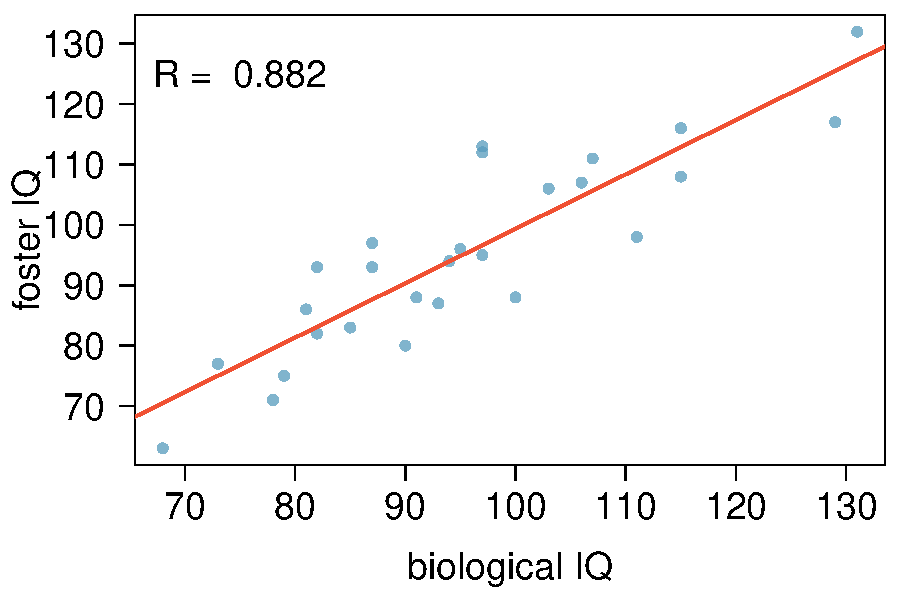
\includegraphics[width=0.7\textwidth]{8-4_inf_lin_reg/figures/twins/twins_IQ}
\end{center}

\end{frame}

%%%%%%%%%%%%%%%%%%%%%%%%%%%%%%%%%%%

\begin{frame}[fragile]
\frametitle{}

\pq{Which of the following is \underline{false}?}

{\footnotesize
\begin{verbatim}
Coefficients:
                 Estimate Std. Error t value Pr(>|t|)    
(Intercept)       9.20760    9.29990   0.990    0.332    
bioIQ             0.90144    0.09633   9.358  1.2e-09

Residual standard error: 7.729 on 25 degrees of freedom
Multiple R-squared: 0.7779,	Adjusted R-squared: 0.769 
F-statistic: 87.56 on 1 and 25 DF,  p-value: 1.204e-09 
\end{verbatim}
}

\begin{enumerate}[(a)]
\item Additional 10 points in the biological twin's IQ is associated with additional 9 points in the foster twin's IQ, on average.
\solnMult{Roughly 78\% of the foster twins' IQs can be accurately predicted by the model.}
\item The linear model is $\widehat{fosterIQ} = 9.2 + 0.9 \times bioIQ$.
\item Foster twins with IQs higher than average IQs tend to have biological twins with higher than average IQs as well.
\end{enumerate}

\end{frame}

%%%%%%%%%%%%%%%%%%%%%%%%%%%%%%%%%%%

\begin{frame}
\frametitle{Testing for the slope}

\pq{Assuming that these 27 twins comprise a representative sample of all twins separated at birth, we would like to test if these data provide convincing evidence that the IQ of the biological twin is a significant predictor of IQ of the foster twin. What are the appropriate hypotheses?}

\begin{enumerate}[(a)]
\item \mathhl{H_0:} $b_0 = 0$; \mathhl{H_A:} $b_0 \ne 0$ 
\item \mathhl{H_0:} $\beta_0 = 0$; \mathhl{H_A:} $\beta_0 \ne 0$ 
\item \mathhl{H_0:} $b_1 = 0$; \mathhl{H_A:} $b_1 \ne 0$ 
\solnMult{ \mathhl{H_0:} $\beta_1 = 0$; \mathhl{H_A:} $\beta_1 \ne 0$ }
\end{enumerate}

\end{frame}

%%%%%%%%%%%%%%%%%%%%%%%%%%%%%%%%%%%

\begin{frame}
\frametitle{Testing for the slope (cont.)}

{\footnotesize
\begin{center}
\begin{tabular}{rrrrr}
  \hline
 & Estimate & Std. Error & t value & Pr($>$$|$t$|$) \\ 
  \hline
(Intercept) & 9.2076 & 9.2999 & 0.99 & 0.3316 \\ 
  bioIQ & 0.9014 & 0.0963 & 9.36 & 0.0000 \\ 
   \hline
\end{tabular}
\end{center}
}

\pause

\begin{itemize}

\item We always use a $t$-test in inference for regression. $\:$ \\

\pause

\Remember{Test statistic, $T = \frac{point~estimate - null~value}{SE}$}

\pause

\item Point estimate = $b_1$ is the observed slope.

\pause

\item $SE_{b_1}$ is the standard error associated with the slope.

\pause

\item Degrees of freedom associated with the slope is $df = n - 2$, where $n$ is the sample size. $\:$ \\
\pause
\Remember{We lose 1 degree of freedom for each parameter we estimate, and in simple linear regression we estimate 2 parameters, $\beta_0$ and $\beta_1$.}

\end{itemize}

\end{frame}

%%%%%%%%%%%%%%%%%%%%%%%%%%%%%%%%%%%

\begin{frame}
\frametitle{Testing for the slope (cont.)}

{\small
\begin{center}
\begin{tabular}{rrrrr}
  \hline
 & Estimate & Std. Error & t value & Pr($>$$|$t$|$) \\ 
  \hline
(Intercept) &  9.2076 & 9.2999 & 0.99 & 0.3316 \\ 
  bioIQ & \orange{0.9014}  &   \green{0.0963} & \orange{9.36} & \textcolor{blue}{0.0000} \\ 
   \hline
\end{tabular}
\end{center}
}

\pause

\begin{eqnarray*}
T &=& \frac{\orange{0.9014} - 0}{\green{0.0963}} = \orange{9.36} \\
\pause
df &=& 27 - 2 = 25 \\
\pause
p-value &=& P(|T| > \orange{9.36}) < \textcolor{blue}{0.01}
\end{eqnarray*}

\end{frame}

%%%%%%%%%%%%%%%%%%%%%%%%%%%%%%%%%%%

\begin{frame}
\frametitle{\% College graduate vs. \% Hispanic in LA}

\dq{What can you say about the relationship between \% college graduate and \% Hispanic in a sample of 100 zip code areas in LA?}

\begin{center}
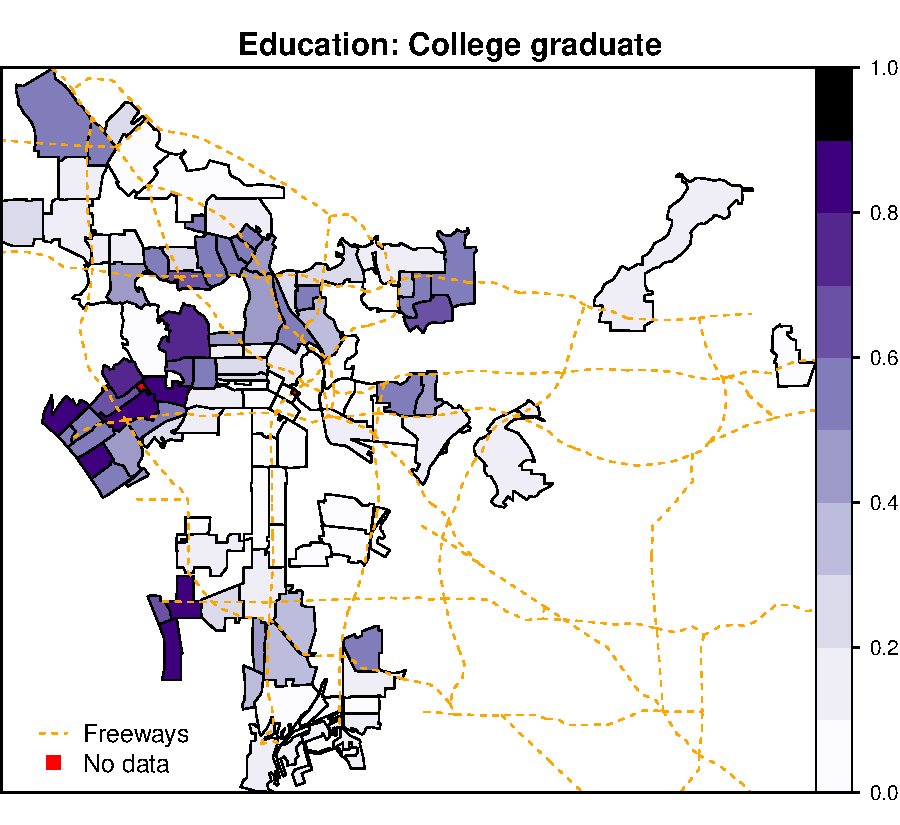
\includegraphics[width=0.53\textwidth]{8-4_inf_lin_reg/figures/la/Prop_EduHigherThan16th}
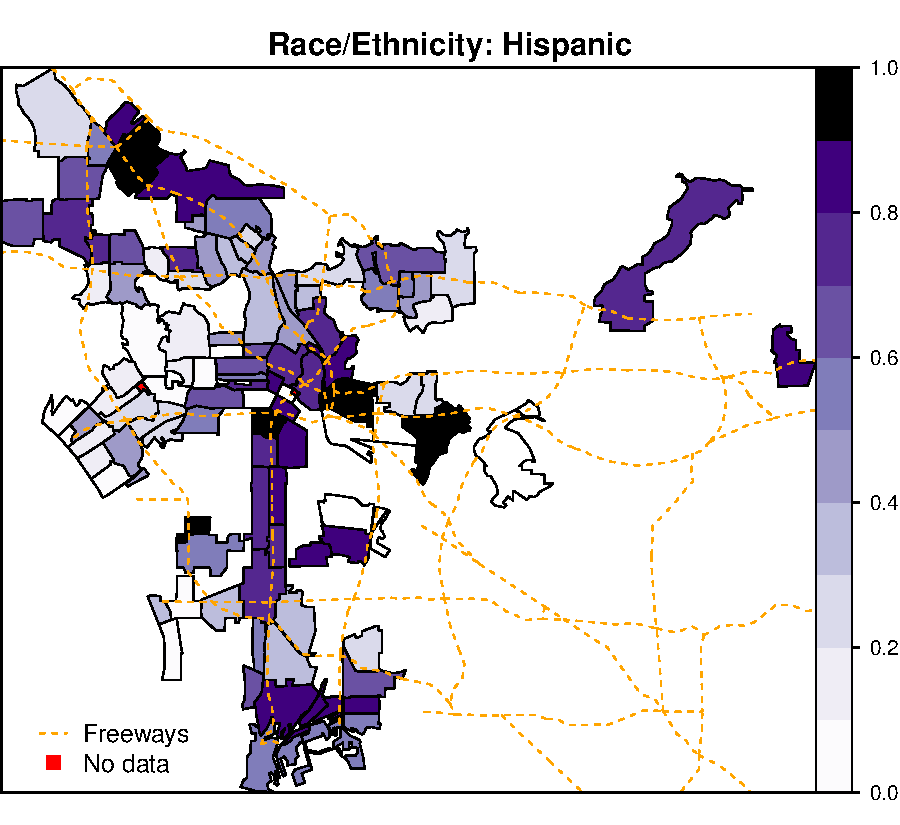
\includegraphics[width=0.53\textwidth]{8-4_inf_lin_reg/figures/la/Prop_RaceEthHispanic}
\end{center}

\end{frame}

%%%%%%%%%%%%%%%%%%%%%%%%%%%%%%%%%%%

\begin{frame}
\frametitle{\% College educated vs. \% Hispanic in LA - another look}

\dq{What can you say about the relationship between of \% college graduate and \% Hispanic in a sample of 100 zip code areas in LA?}

\begin{center}
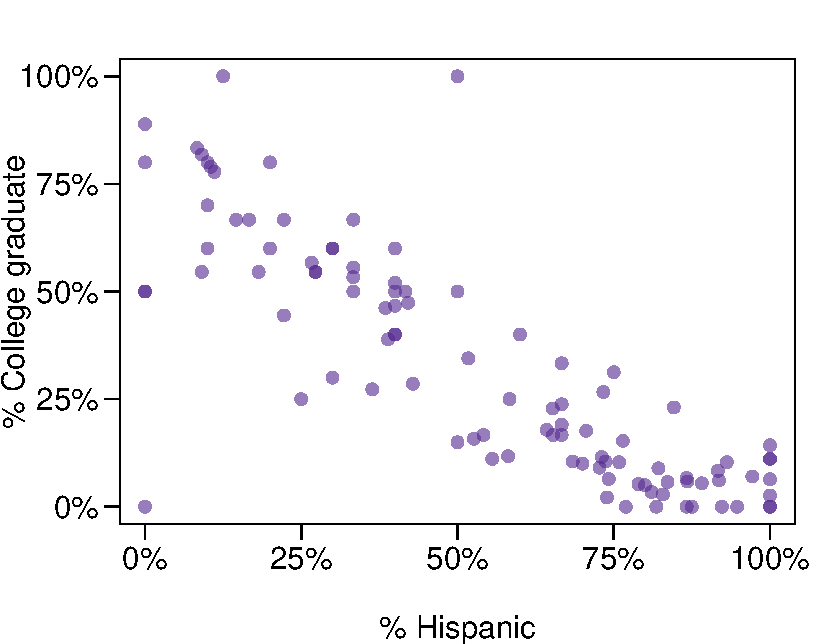
\includegraphics[width=0.7\textwidth]{8-4_inf_lin_reg/figures/la/la}
\end{center}

\end{frame}

%%%%%%%%%%%%%%%%%%%%%%%%%%%%%%%%%%%

\begin{frame}
\frametitle{\% College educated vs. \% Hispanic in LA - linear model}

\pq{Which of the below is the best interpretation of the slope?}

{\small
\begin{center}
\begin{tabular}{rrrrr}
  \hline
 & Estimate & Std. Error & t value & Pr($>$$|$t$|$) \\ 
  \hline
(Intercept) & 0.7290 & 0.0308 & 23.68 & 0.0000 \\ 
 \%Hispanic & -0.7527 & 0.0501 & -15.01 & 0.0000 \\ 
   \hline
%   &&&&$df$ = 98 \\
\end{tabular}
\end{center}
}

\begin{enumerate}[(a)]
\item A 1\% increase in Hispanic residents in a zip code area in LA is associated with a 75\% decrease in \% of college grads.
\solnMult{A 1\% increase in Hispanic residents in a zip code area in LA is associated with a 0.75\% decrease in \% of college grads.}
\item An additional 1\% of Hispanic residents decreases the \% of college graduates in a zip code area in LA by 0.75\%.
\item In zip code areas with no Hispanic residents, \% of college graduates is expected to be 75\%.
\end{enumerate}

\end{frame}

%%%%%%%%%%%%%%%%%%%%%%%%%%%%%%%%%%%

\begin{frame}
\frametitle{\% College educated vs. \% Hispanic in LA - linear model}

\dq{Do these data provide convincing evidence that there is a statistically significant relationship between \% Hispanic and \% college graduates in zip code areas in LA?}

{\small
\begin{center}
\begin{tabular}{rrrrr}
  \hline
 & Estimate & Std. Error & t value & Pr($>$$|$t$|$) \\ 
  \hline
(Intercept) & 0.7290 & 0.0308 & 23.68 & 0.0000 \\ 
  hispanic & -0.7527 & 0.0501 & -15.01 & 0.0000 \\ 
   \hline
%   &&&&$df$ = 98 \\
\end{tabular}
\end{center}
}
\soln{\only<2->{Yes, the p-value for \% Hispanic is low, indicating that the data provide convincing evidence that the slope parameter is different than 0.
}}

$\:$ \\

\dq{How reliable is this p-value if these zip code areas are not randomly selected?}
\soln{\only<3->{Not very...
}}

\end{frame}

%%%%%%%%%%%%%%%%%%%%%%%%%%%%%%%%%%%

\subsection{CI for the slope}

%%%%%%%%%%%%%%%%%%%%%%%%%%%%%%%%%%%

\begin{frame}
\frametitle{Confidence interval for the slope}

\pq{{\small Remember that a confidence interval is calculated as $point~estimate \pm ME$ and the degrees of freedom associated with the slope in a simple linear regression is $n - 2$. Which of the below is the correct 95\% confidence interval for the slope parameter? Note that the model is based on observations from 27 twins.}}

{\footnotesize
\begin{center}
\begin{tabular}{rrrrr}
  \hline
 & Estimate & Std. Error & t value & Pr($>$$|$t$|$) \\ 
  \hline
(Intercept) & 9.2076 & 9.2999 & 0.99 & 0.3316 \\ 
  bioIQ & 0.9014 & 0.0963 & 9.36 & 0.0000 \\ 
   \hline
\end{tabular}
\end{center}
}

\vspace{-0.5cm}

\twocol{0.4}{0.6}
{
\begin{enumerate}[(a)]
\item $9.2076 \pm 1.65 \times 9.2999$
\solnMult{ $0.9014 \pm 2.06 \times 0.0963$}
\item $0.9014 \pm 1.96 \times 0.0963$
\item $9.2076 \pm 1.96 \times 0.0963$
\end{enumerate}
}
{
\soln{\onslide<2->{\orange{
\begin{eqnarray*}
\pause
n &=& 27 \qquad df = 27 - 2 = 25 \\
\pause
95\%:~t^\star_{25} &=& 2.06 \\
\pause
0.9014 &\pm& 2.06 \times 0.0963 \\
\pause
(0.7 &,& 1.1)
\end{eqnarray*}
}}}}

\end{frame}

%%%%%%%%%%%%%%%%%%%%%%%%%%%%%%%%%%%

\begin{frame}
\frametitle{Recap}

\begin{itemize}

\item Inference for the slope for a single-predictor linear regression model:
\pause
\begin{itemize}
\item Hypothesis test:
\[ T = \frac{b_1 - null~value}{SE_{b_1}} \qquad df = n - 2 \]
\pause
\item Confidence interval:
\[ b_1 \pm t^\star_{df = n - 2} SE_{b_1} \]
\end{itemize}

\pause

\item The null value is often 0 since we are usually checking for \hl{any} relationship between the explanatory and the response variable.

\pause

\item The regression output gives $b_1$, $SE_{b_1}$, and \hl{two-tailed} p-value for the $t$-test for the slope where the null value is 0.

\pause

\item We rarely do inference on the intercept, so we'll be focusing on the estimates and inference for the slope.

\end{itemize}

\end{frame}

%%%%%%%%%%%%%%%%%%%%%%%%%%%%%%%%%%%


\begin{frame}
\frametitle{Caution}

\begin{itemize}

\item Always be aware of the type of data you're working with: random sample, non-random sample, or population.

\pause

\item Statistical inference, and the resulting p-values, are meaningless when you already have population data.

\pause

\item If you have a sample that is non-random (biased), inference on the results will be unreliable.

\pause

\item The ultimate goal is to have independent observations.

\end{itemize}

\end{frame}

%%%%%%%%%%%%%%%%%%%%%%%%%%%%%%%%%%%